%%%%%%%%%%%%%%%%%%%%%%%%%%%%%%%%%%%%%%%%%%%%%%%%%%%%%%%%%%%%%%%%%%%%%%%%%%%%%
%%%%%%                                                                  %%%%% 
%%%%%%          Maqueta de memòria TFC/PFC de l'EETAC                   %%%%% 
%%%%%%                                                                  %%%%% 
%%%%%%%%%%%%%%%%%%%%%%%%%%%%%%%%%%%%%%%%%%%%%%%%%%%%%%%%%%%%%%%%%%%%%%%%%%%%%
%%%%%%%%%%%%%%%%%%%%%%%%%%%%%%%%%%%%%%%%%%%%%%%%%%%%%%%%%%%%%%%%%%%%%%%%%%%%%
%%                                                                         %%
%%          Autor: Xavier Prats i Menéndez (xavier.prats@upc.edu)          %% 
%%                  Technical University of Catalonia (UPC)                %%
%%                                                                         %%
%%%%%%%%%%%%%%%%%%%%%%%%%%%%%%%%%%%%%%%%%%%%%%%%%%%%%%%%%%%%%%%%%%%%%%%%%%%%%
%%      This work is licensed under the Creative Commons  Attribution-     %%
%%   -Noncommercial-Share Alike 3.0 Spain License. To view a copy of this  %% 
%%    license, visit http://creativecommons.org/licenses/by-nc-sa/3.0/es/  %%
%%    or send a letter to Creative Commons, 171 Second Street, Suite 300,  %%
%%                  San Francisco,California, 94105, USA.                  %%
%%%%%%%%%%%%%%%%%%%%%%%%%%%%%%%%%%%%%%%%%%%%%%%%%%%%%%%%%%%%%%%%%%%%%%%%%%%%%
%% Versió 2.1 - Juliol 2012                                                %%
%%%%%%%%%%%%%%%%%%%%%%%%%%%%%%%%%%%%%%%%%%%%%%%%%%%%%%%%%%%%%%%%%%%%%%%%%%%%%

%%% NOTA: els seguents packages son necessaris per utilitzar la
%%%       plantilla seguent:
%%%       ifthen,calc,helvet,pslatex,fancyhdr,nextpage,subfigure,tocloft,graphicx,url

%%% NOTA: Es possible que algunes distribuicions Linux o Windows.
%%%       no portin aquests paquets instal·lats per defecte.
%%%       En aquest cas els haureu d'instal·lar manualment.


%%%%%%%%%%%%%%%%%%%%%%%%%%%%%%%%%%%%%%%%%%%%%%%%%%%%%%%%%%%%%%%%%%%%%%%%%%%%%
% 1- INICIALITZACIÓ
%%%%%%%%%%%%%%%%%%%%%%%%%%%%%%%%%%%%%%%%%%%%%%%%%%%%%%%%%%%%%%%%%%%%%%%%%%%%%

\documentclass[english,final]{setup/eetac_tfc_pfc}
%% * OPCIONS A CONFIGURAR al \documentclass
%%    - Estat del document: final o draft
%%      NOTA: Draft no inserta les figures i marca només l'espai que
%%      ocupen. També s'indica quan el text sobrepassa els marges.
%%      Draft és molt útil per compilar ràpid el document si no és important
%%      en aquell moment visualitzar les figures.
%%    - Idioma PRINCIPAL del document: catalan, spanish, english, french...

\usepackage[english]{babel}
%%  * INCLOURE TOTS ELS IDIOMES QUE S'USARAN EN EL DOCUMENT
%%    NOTA: per canviar d'idioma al mig del document usar:
%%          \selectlanguage{nom_idioma}
%%%%%%%%%%%%%%%%%%%%%%%%%%%%%%%%%%%%%%%%%%%%%%%%%%%%%%%%%%%%%%%%%%%%%%%%%%%%%

%%%%%%%%%%%%%%%%%%%%%%%%%%%%%%%%%%%%%%%%%%%%%%%%%%%%%%%%%%%%%%%%%%%%%%%%%%%%%
% 2- CÀRREGA DE PAQUETS ADICIONALS (OPCIONALS)
%%%%%%%%%%%%%%%%%%%%%%%%%%%%%%%%%%%%%%%%%%%%%%%%%%%%%%%%%%%%%%%%%%%%%%%%%%%%%

%%% NOTA: Es possible que algunes distribuicions Linux o Windows.
%%%       no portin aquests paquets instal·lats per defecte.
%%%       En aquest cas els haureu d'instal·lar manualment.

%% El paquet inputenc és extramadament útil. 
%% Permet escriure els accents directament amb l'editor de texte
%% sense haver de fer coses com per exemple: introducci\'o
%% Heu d'especificar la codificació de caracters que utilitzeu pel
%% vostre fitxer (en aquest exemple utf8)
\usepackage[utf8]{inputenc}

%% Símbols matemàtics de la American Mathematical Society
\usepackage{amssymb, amsmath, amsfonts}  

%% El paquet array proporciona eines molt útils a l'hora de fer 
%% equacions amb matrius
\usepackage{array}             

%% Paquet que permet fer taules fusionant cel·les de files consecutives
\usepackage{multirow}          

%% Paquet molt útil en cas de tenir taules molt llargues que 
%   ocupin vàries pàgines
\usepackage{longtable}          

%% Permet canviar els colors del document
\usepackage{color,colortbl}

%% Paquet molt útil que permet activar links en el PDF final.
\usepackage[
  	% CUSTOM PDF 
  	pdfauthor={Fernando Román García},
  	pdftitle={Master thesis - Fernando Román García},
	pdfsubject={An enhanced SleuthKit GUI for digital forensics},
	pdfkeywords={digital, forensics, sleuth, kit, GUI},
	%
  	pdfcreator={EETAC-UPC},
	pdfproducer={LaTeX, dvipdf},
	pdfdisplaydoctitle=true,
  	plainpages=false,
	linktocpage=true,
	colorlinks=true,
  	linkcolor=blue,
	citecolor=blue,
	urlcolor=blue,
	hyperfootnotes=false,
  	pagebackref=true,
	pdfpagelabels=true,
	pdfpagemode=UseOutlines,
]{hyperref} 

%% NOTA IMPORTANT!:
%% Per tal que hyperef funcioni correctament amb els capitols o seccions no
%% numerats (\chapter*{}), com per exemple introducció, conclusions i
%% bibliografia cal posar les dues comandes seguents ABANS del \chapter*{} en
%% questió
%\cleardoublepage \phantomsection

%% Permet trencar links URL. 
%% Atenció! afegir aquest paquet DESPRES del hyperref!!
\usepackage{breakurl} 

%% Permet arranjar matricialment multiples figures
%% NOTA: afegir aquest paquet DESPRES del hyperref!!
%%       Si no es desitja utilitzar aquest paquet, comentar la linia seguent
%%       i anar TAMBE al fitxer de classe (eetac_tfc_pfc.cls) per substituir: 
%%       \RequirePackage[subfigure]{tocloft}  per  \RequirePackage{tocloft}
\usepackage{subfigmat}

% Custom packages
\usepackage{xparse}
\usepackage{listings}
\usepackage{rotating}
\usepackage{pdflscape}
\usepackage{wrapfig}
\usepackage{etoolbox}
\usepackage{makecell}
\usepackage{lscape}

%%%%%%%%%%%%%%%%%%%%%%%%%%%%%%%%%%%%%%%%%%%%%%%%%%%%%%%%%%%%%%%%%%%%%%%%%%%%%
% 3- DOCUMENT
%%%%%%%%%%%%%%%%%%%%%%%%%%%%%%%%%%%%%%%%%%%%%%%%%%%%%%%%%%%%%%%%%%%%%%%%%%%%%

%%% Configuració de les dades i variables boleanes rellevants del document:
%%%%%%%%%%%%%%%%%%%%%%%%%%%%%%%%%%%%%%%%%%%%%%%%%%%%%%%%%%%%%%%%%%%%%%%%%%%%%
%%%%%%                                                                  %%%%% 
%%%%%%       Fitxer de dades per la memoria TFC/PFC de l'EETAC          %%%%% 
%%%%%%                                                                  %%%%% 
%%%%%%%%%%%%%%%%%%%%%%%%%%%%%%%%%%%%%%%%%%%%%%%%%%%%%%%%%%%%%%%%%%%%%%%%%%%%%
%%%%%%%%%%%%%%%%%%%%%%%%%%%%%%%%%%%%%%%%%%%%%%%%%%%%%%%%%%%%%%%%%%%%%%%%%%%%%
%%                                                                         %%
%%          Autor: Xavier Prats i Menendez (xavier.prats@upc.edu)          %% 
%%                  Technical University of Catalonia (UPC)                %%
%%                                                                         %%
%%%%%%%%%%%%%%%%%%%%%%%%%%%%%%%%%%%%%%%%%%%%%%%%%%%%%%%%%%%%%%%%%%%%%%%%%%%%%
%%      This work is licensed under the Creative Commons  Attribution-     %%
%%   -Noncommercial-Share Alike 3.0 Spain License. To view a copy of this  %% 
%%    license, visit http://creativecommons.org/licenses/by-nc-sa/3.0/es/  %%
%%    or send a letter to Creative Commons, 171 Second Street, Suite 300,  %%
%%                  San Francisco,California, 94105, USA.                  %%
%%%%%%%%%%%%%%%%%%%%%%%%%%%%%%%%%%%%%%%%%%%%%%%%%%%%%%%%%%%%%%%%%%%%%%%%%%%%%
%% Versio 2.1 - Juliol 2012                                                %%
%%%%%%%%%%%%%%%%%%%%%%%%%%%%%%%%%%%%%%%%%%%%%%%%%%%%%%%%%%%%%%%%%%%%%%%%%%%%%

%%%%%%%%%%%%%%%%%%%%%%%%%%%%%%%%%%%%%%%%%%%%%%%%%%%%%%%%%%%%%%%%%%%%%%%%%%%%%%%
%%  VARIABLES A CONFIGURAR                                                  %%%
%%%%%%%%%%%%%%%%%%%%%%%%%%%%%%%%%%%%%%%%%%%%%%%%%%%%%%%%%%%%%%%%%%%%%%%%%%%%%%%

%% - Projecte o Treball de Fi de Carrera?
%%      PFC = true   -> Projecte de Fi de Carrera
%%      PFC = false  -> Treball  de Fi de Carrera
\setboolean{PFC}{false}

%% - Escollir la titulació
%\titulacio{Enginyeria Tècnica Aeronàutica, especialitat Aeronavegació}
%\titulacio{Enginyeria T\`ecnica de Telecomunicaci\'o, especialitat Sistemes de Telecomunicaci\'o}
%\titulacio{Enginyeria T\`ecnica de Telecomunicaci\'o, especialitat Telem\`atica}
%\titulacio{Enginyeria de Telecomunicaci\'o (segon cicle)}
% Modificació respecte a la versió 2.1 - Iván Padilla Montero - Juliol 2014
%\titulacio{Grau en Enginyeria d'Aeronavegaci\'o}
%\titulacio{Grau en Enginyeria d'Aeroports}
%\titulacio{Grau en Enginyeria Telemàtica}
%\titulacio{Grau en Enginyeria de Sistemes de Telecomunicació}
\titulacio{Master's degree in Applied Telecommunications and Engineering Management (MASTEAM)}

%% - Configurar els idiomes del document
%% Si l'idioma PRINCIPAL del document es l'angles, posar aquesta variable a true
\setboolean{Leng}{true}

%% Escollir entre catala i castella (idioma principial, o nomes pel resum en cas que l'idioma principal sigui anglès)
%%  catala = true   -> idioma principal (o només resum) en Català
%%  catala = false  -> idioma principal (o només resum) en Castella
\setboolean{Lcat}{false}

%% Titol del document en l'idioma principal del document 
\titol{An enhanced SleuthKit GUI for digital forensics}

%% Titol del document en anglès (Per l'apartat overview)
\titolE{An enhanced SleuthKit GUI for digital forensics}

%% Titol del document en catala/castella (Per l'apartat resum)
\titolC{An enhanced SleuthKit GUI for digital forensics}


%% - Nombre d'autors del TFC/PFC?
%%      UNautor = true   Un sol autor
%%      UNautor = false  Més d'un autor
\setboolean{UNautor}{true}

%% - Nom del(s) Autor(s) del document
%% NOTA: En cas de mes d'un autor cal posar la comana \and entre els
%%        noms dels autors
\autor{Fernando Román García}

%% - Nombre de directors del TFC/PFC. Tipicament 1 o 2
%%      UNdirector = true   Un sol director
%%      UNdirector = false  Dos directors
\setboolean{UNdirector}{true}

%% - Nom del Director del TFC/PFC
\director{Juan Hernández Serrano}

%% - Nom del segon director en cas de tenir-lo:
\segonDirector{Nom2 Cognoms2}


%% - Es vol incloure una dedicatoria?
%%      dedicatoria = true   -> S'afegeix una pagina amb \textDedicatoria
%%      dedicatoria = true   -> No s'afegeix dedicatoria
%% NOTA: no confondre dedicatòria amb agraïments. Una dedicatoria sol ser
%%       un missatge curt d'una o dues frases màxim a la persona, o persones
%%       a les quals es dedica el treball. 
%%       Els agraïments poden ser extensos i l'autor pot agraïr a diverses
%%       persones coses diferents en funció de l'ajuda rebuda, per exemple. 
%%       Si es volen incloure agraïments, fer-ho al fitxer de la 
%%       memòria creant una secció nova amb  \chapter*{Agraïments}
\setboolean{dedicatoria}{false}
\textDedicatoria{Escriure aqui \\ la dedicatòria}

%% - Es vol incloure una pagina d'index de figures?
\setboolean{paginaLOF}{true}  % List of Figures

%% - Es vol incloure una pagina d'index de taules?
\setboolean{paginaLOT}{true}  % List of Tables 

%% - El projecte ha estat supervisat per alguna persona externa? 
%%   (NOMES en cas de practiques en empresa)
%%      supervisor = true    -> Hi ha un supervisor
%%      supervisor = false   -> No hi ha un supervisor
\setboolean{supervisor}{false}

%% NOMES en el cas de practiques en empresa (supervisor=true) s'han de 
%% configurar les variables seguents: 

%% Supervisor del TFC/PFC 
\supervisor{Nom del Supervisor}

%% - Es vol incloure el logotip de l'empresa?
%%   En el cas que el TFC/PFC s'hagi fet en règim d'intercanvi amb una
%%   empresa, es pot afegir el seu logotip a la cantonada superior
%%   dreta de la portada. En aquest cas:
%%   - posar logo=true
%%   - posar el path de la imatge i l'alçada del logo a \mylogo
\setboolean{logo}{true}
\mylogo{./setup/EETAC-positiu}{1.5cm}
  

%%% Configuració de MACROS o ENTORNS (opcionals) definides per l'usuari:
%%%%%%%%%%%%%%%%%%%%%%%%%%%%%%%%%%%%%%%%%%%%%%%%%%%%%%%%%%%%%%%%%%%%%%%%%%%%%
%%%%%%                                                                  %%%%% 
%%%%%%    Fitxer de macros d'usuari per la memoria TFC/PFC de l'EETAC   %%%%% 
%%%%%%                                                                  %%%%% 
%%%%%%%%%%%%%%%%%%%%%%%%%%%%%%%%%%%%%%%%%%%%%%%%%%%%%%%%%%%%%%%%%%%%%%%%%%%%%
%%%%%%%%%%%%%%%%%%%%%%%%%%%%%%%%%%%%%%%%%%%%%%%%%%%%%%%%%%%%%%%%%%%%%%%%%%%%%
%%                                                                         %%
%%         Author: Xavier Prats i Menendez (xavier.prats@upc.edu)          %% 
%%                  Technical University of Catalonia (UPC)                %%
%%                                                                         %%
%%%%%%%%%%%%%%%%%%%%%%%%%%%%%%%%%%%%%%%%%%%%%%%%%%%%%%%%%%%%%%%%%%%%%%%%%%%%%
%%      This work is licensed under the Creative Commons  Attribution-     %%
%%   -Noncommercial-Share Alike 3.0 Spain License. To view a copy of this  %% 
%%    license, visit http://creativecommons.org/licenses/by-nc-sa/3.0/es/  %%
%%    or send a letter to Creative Commons, 171 Second Street, Suite 300,  %%
%%                  San Francisco,California, 94105, USA.                  %%
%%%%%%%%%%%%%%%%%%%%%%%%%%%%%%%%%%%%%%%%%%%%%%%%%%%%%%%%%%%%%%%%%%%%%%%%%%%%%
%% Versio 1.5 - Juliol 2010                                                %%
%%%%%%%%%%%%%%%%%%%%%%%%%%%%%%%%%%%%%%%%%%%%%%%%%%%%%%%%%%%%%%%%%%%%%%%%%%%%%


%%% Xevi's macros for vectors and matrices:

%\newcommand{\ve}[1]{\mbox{\boldmath$#1$}}          
\newcommand{\ve}[1]{\vec{#1}}  
\newcommand{\ma}[1]{\mbox{\boldmath$\mathcal{#1}$}}

%%% Xevi's macros for brackets:
\newcommand{\lp}{\left(}
\newcommand{\lc}{\left[}
\newcommand{\lcl}{\left\{}
\newcommand{\rp}{\right)}
\newcommand{\rc}{\right]}
\newcommand{\rcl}{\right\}}

%%% Xevi's new environment for HIPOTESIS
\newcounter{num_hyp}
\newenvironment{hyp}[2]{
        \refstepcounter{num_hyp}
        \vspace*{2.5ex}
        {\noindent \bf\sffamily HYPOTHESIS #1 : #2} \\
        \sl
}
        {\vspace{1ex}
}

\newcommand{\SUMhyp}[2]{
 {\sffamily HYPOTHESIS #1 : #2} 
}

\newcommand{\icon}[2]{%
	$\null\mathsurround=0pt$%
	\includegraphics[height=\dimexpr\fontdimen22\textfont2+1ex\relax]{#1}
	\textbf{#2.}\space}

\def\CC{{C\nolinebreak[4]\hspace{-.05em}\raisebox{.3ex}{\small\bf ++}\space}}

\newcommand{\approxtext}[1][]{%
	\ensuremath{\stackrel{\text{#1}}{\approx}}
}


%% CUSTOM SETTINGS

\def\arraystretch{2}

\renewcommand\theadalign{bc}
\renewcommand\theadfont{\bfseries}
\renewcommand\theadgape{\Gape[4pt]}
\renewcommand\cellgape{\Gape[4pt]}
  

%%% Configuració manual de les regles d'hyphenation:
%%%%%%%%%%%%%%%%%%%%%%%%%%%%%%%%%%%%%%%%%%%%%%%%%%%%%%%%%%%%%%%%%%%%%%%%%%%%%
%%%%%%                                                                  %%%%% 
%%%%%%    Fitxer de hyphenation per la memoria TFC/PFC de l'EETAC       %%%%% 
%%%%%%                                                                  %%%%% 
%%%%%%%%%%%%%%%%%%%%%%%%%%%%%%%%%%%%%%%%%%%%%%%%%%%%%%%%%%%%%%%%%%%%%%%%%%%%%
%%%%%%%%%%%%%%%%%%%%%%%%%%%%%%%%%%%%%%%%%%%%%%%%%%%%%%%%%%%%%%%%%%%%%%%%%%%%%
%%                                                                         %%
%%         Author: Xavier Prats i Menendez (xavier.prats@upc.edu)          %% 
%%                  Technical University of Catalonia (UPC)                %%
%%                                                                         %%
%%%%%%%%%%%%%%%%%%%%%%%%%%%%%%%%%%%%%%%%%%%%%%%%%%%%%%%%%%%%%%%%%%%%%%%%%%%%%
%%      This work is licensed under the Creative Commons  Attribution-     %%
%%   -Noncommercial-Share Alike 3.0 Spain License. To view a copy of this  %% 
%%    license, visit http://creativecommons.org/licenses/by-nc-sa/3.0/es/  %%
%%    or send a letter to Creative Commons, 171 Second Street, Suite 300,  %%
%%                  San Francisco,California, 94105, USA.                  %%
%%%%%%%%%%%%%%%%%%%%%%%%%%%%%%%%%%%%%%%%%%%%%%%%%%%%%%%%%%%%%%%%%%%%%%%%%%%%%
%% Versio 1.5 - Juliol 2010                                                %%
%%%%%%%%%%%%%%%%%%%%%%%%%%%%%%%%%%%%%%%%%%%%%%%%%%%%%%%%%%%%%%%%%%%%%%%%%%%%%

\hyphenation{Cas-tell-de-fels}
\hyphenation{EETAC}
  

%%% Configurations of programming languages highlights 
% Listing toc configuration %%%%%%%%%%%%%%%%%%%%%%%%%%%%%%%%%%%%%%%%%%%%%%%%%%%%

\let\Chapter\chapter
\def\chapter{\addtocontents{lol}{\protect\addvspace{10pt}}\Chapter}

% Colors %%%%%%%%%%%%%%%%%%%%%%%%%%%%%%%%%%%%%%%%%%%%%%%%%%%%%%%%%%%%%%%%%%%%%%%

% Green
\definecolor{dkgreen}{rgb}{0,0.6,0}
\definecolor{deepgreen}{rgb}{0,0.5,0}
\definecolor{olivedrab}{RGB}{94,140,34}

% Gray
\definecolor{sirocco}{RGB}{114,128,131}
\definecolor{gray}{rgb}{0.5,0.5,0.5}

\definecolor{mauve}{rgb}{0.58,0,0.82}
\definecolor{deepblue}{rgb}{0,0,0.5}
\definecolor{deepred}{rgb}{0.6,0,0}

\definecolor{deepviolet}{RGB}{121, 8, 125}

% Blue
\definecolor{gigas}{RGB}{72, 62, 170}
\definecolor{pictonblue}{RGB}{62, 193, 233}
\definecolor{turquoiseblue}{RGB}{64, 224, 208}
\definecolor{bluebayoux}{RGB}{87,115,131}
\definecolor{funblue}{RGB}{25,78,155}

\definecolor{saffron}{rgb}{0.372,0.211,0.988}
\definecolor{rawsienna}{rgb}{0.819,0.576,0.255}

\definecolor{brightedred}{RGB}{161,0,0}


% Custom macros %%%%%%%%%%%%%%%%%%%%%%%%%%%%%%%%%%%%%%%%%%%%%%%%%%%%%%%%%%%%%%%%


\lstdefinestyle{defaults}{
	basicstyle=\footnotesize\ttfamily,
	captionpos=b,
	aboveskip=3mm,
	belowskip=3mm,
	showstringspaces=false,
	columns=flexible,
	numbers=left,
	numberstyle=\footnotesize,
	breaklines=true,
	breakatwhitespace=true,
	tabsize=3,
	escapechar=\%,
}
\newcommand{\lstcustomdefaults}{
	\setkeys{lst}{
		style=defaults
	}
}
\newcommand{\newproglanguage}[2]{
	\expandafter\newcommand\csname #1style\endcsname[1][]{
		#2
		\lstcustomdefaults
		\setkeys{lst}{##1}
	}

	\lstnewenvironment{#1}[1][]
	{
		\expandafter\csname #1style\endcsname
		\lstset{##1}
	}
	{}
	
	\expandafter\DeclareDocumentCommand\csname #1external\endcsname
	{ O{} m }
	{
		\expandafter\csname #1style\endcsname
		\lstinputlisting[##1]{##2}
	}
	
	\expandafter\newcommand\csname #1inline\endcsname
	[1]{{\expandafter\csname #1style\endcsname\lstinline!##1!}}
}

%% Code figure
\newenvironment{codefigure}{
	\begin{quote}
}
{
	\end{quote}
}

%% Terminal
\newcommand{\termuser}{user}
\newcommand{\termhost}{host}
\newcommand{\termdir}{/home/user}
\newcommand{\terminalcmd}[1][]{%
\textbf{%
	{\color{olivedrab} \termuser\text{@}\termhost:}%
	{\color{funblue} \termdir}}\$ #1
}

\lstnewenvironment{terminal}[1][]{
	\lstset{
		style=defaults,
		backgroundcolor=\color{black},
		basicstyle=\footnotesize\ttfamily\color{white},
		captionpos=b,
		numbers=none,
		aboveskip=3mm,
		belowskip=3mm,
		framexleftmargin=6pt,  xleftmargin=6pt,
		framexrightmargin=6pt, xrightmargin=6pt, 
		framextopmargin=6pt,
		framexbottommargin=6pt,
		frame=tb, framerule=0pt,
		showstringspaces=false,
		columns=flexible,
		breaklines=true,
		breakatwhitespace=true,
		tabsize=3,
		% Language settings
		numberstyle=\tiny\color{gray},
		commentstyle=\color{dkgreen},
		stringstyle=\color{red},
		% Classes
		classoffset=0,
		keywordstyle=\color{gigas},
		% Classes
		classoffset=1,
		keywords={System, String},
		keywordstyle=\color{deepviolet}\itshape,
	}
	\setkeys{lst}{#1}
}{}

\newcommand{\asdf}[1]{\textbf{#1}}

%% Bash code
\newenvironment{bashcode}{\endgraf\centering\itshape\bfseries}{}


% Style highlighting %%%%%%%%%%%%%%%%%%%%%%%%%%%%%%%%%%%%%%%%%%%%%%%%%%%%%%%%%%%

%% Java
\newproglanguage{java}{
	\lstset{
		language=Java,
		% Language settings
		numberstyle=\tiny\color{gray},
		commentstyle=\color{dkgreen},
		stringstyle=\color{red},
		% Classes
		classoffset=0,
		keywordstyle=\color{gigas},
		% Classes
		classoffset=1,
		keywords={System, String},
		keywordstyle=\color{deepviolet}\itshape,
	}
}

%% Python
\newproglanguage{python}{
	\lstset{
		language=Python,
		otherkeywords={self},             	 % Add keywords here
		keywordstyle=\color{deepblue},
		emph={
			__init__,
			TestApp,
			App,
			Button
		},          				    	 % Custom highlighting
		emphstyle=\color{deepviolet}\itshape,% Custom highlighting style
		stringstyle=\color{red},
	}
}

%% C++
\newproglanguage{cpp}{
	\lstset{
		language=C++,
		% Language settings
		commentstyle=\color{dkgreen}\ttfamily,
		identifierstyle=\color{black},
		stringstyle=\color{red}\ttfamily,
		morecomment=[l][\color{magenta}]{\#},
		% Syntax keywords
		classoffset=0,
		keywordstyle=\color{gigas},
		% Classes
		classoffset=1,
		keywordstyle=\color{deepviolet}\itshape,
	}
}


%% JavaScript
\lstdefinelanguage{JavaScript}{
	% Language settings
	sensitive=true,
	% Keywords
	classoffset=0,
	keywords={typeof, new, true, false, catch, function, return,
		null, catch, switch, var, if, in, while, do, else, case,
		break, const, let, class, export, boolean, throw, implements,
		default, import, this, extends},
	% Classes
	classoffset=1,
	keywords={Math, BrowserWindow, Menu, MenuItem, Rx, Observable, Date,
			  module, exports},
	% Comments
	comment=[l]{//},
	morecomment=[s]{/*}{*/},
	% Strings
	morestring=[b]',
	morestring=[b]",
}
\newproglanguage{js}{
	\lstset{
		language=JavaScript,
		% General theme
		commentstyle=\color{dkgreen}\ttfamily,
		identifierstyle=\color{black},
		stringstyle=\color{red}\ttfamily,
		% Syntax keywords
		classoffset=0,
		keywordstyle=\color{gigas},
		% Classes
		classoffset=1,
		keywordstyle=\color{deepviolet}\itshape,
	}
}

%% JavaScript
\lstdefinelanguage{TypeScript}{
	% Language settings
	language=JavaScript,
	sensitive=true,
	% Keywords
	classoffset=0,
	keywords={typeof, new, true, false, catch, function, return,
		null, catch, switch, var, if, in, while, do, else, case,
		break, const, let, class, export, throw, implements,
		default, import, this, extends,
		%
		interface, type, constructor, public, private, declare, module},
	% Classes
	classoffset=1,
	keywords={Math, BrowserWindow, Menu, MenuItem, Rx, Observable, Date,
		%
		string, Array, number, boolean, Buffer, void, any, Store},
	% Comments
	comment=[l]{//},
	morecomment=[s]{/*}{*/},
	% Strings
	morestring=[b]',
	morestring=[b]",
}
\newproglanguage{ts}{
	\lstset{
		language=TypeScript,
		% General theme
		commentstyle=\color{dkgreen},
		identifierstyle=\color{black},
		stringstyle=\color{red},
		% Syntax keywords
		classoffset=0,
		keywordstyle=\color{gigas},
		% Classes
		classoffset=1,
		keywordstyle=\color{deepviolet}\itshape,
	}
}

%% JSX
\lstdefinelanguage{JSX}{
	% Language settings
	alsoletter={<, >, \/},
	sensitive=true,
	% Keywords
	classoffset=0,
	keywords={typeof, new, true, false, catch, function, return,
		null, catch, switch, var, if, in, while, do, else, case,
		break, const, let, class, export, boolean, throw, implements,
		default, import, this, extends},
	% Classes
	classoffset=1,
	keywords={Math, BrowserWindow, Menu, MenuItem, Rx, Observable, Date},
	% HTML
	classoffset=2,
	keywords={<div>,<\/div>,/>},
	% Comments
	comment=[l]{//},
	morecomment=[s]{/*}{*/},
	% Strings
	morestring=[b]',
	morestring=[b]",
}
\newproglanguage{jsx}{
	\lstset{
		language=JSX,
		% General theme
		commentstyle=\color{dkgreen},
		identifierstyle=\color{black},
		stringstyle=\color{red},
		% Syntax keywords
		classoffset=0,
		keywordstyle=\color{gigas},
		% Classes
		classoffset=1,
		keywordstyle=\color{deepviolet}\itshape,
		% HTML
		classoffset=2,
		moredelim=*[s][{\color{saffron}}]{<}{>},
		keywordstyle=\color{saffron},
	}
}

%% Haxe
\lstdefinelanguage{Haxe}{
	% General theme
	sensitive=true,
	% Syntax keywords
	classoffset=0,
	keywords={class, static, public, function, var},
	% Classes
	classoffset=1,
	keywords={String, Void},
	% Comments
	comment=[l]{//},
	morecomment=[s]{/*}{*/},
	% Strings
	morestring=[b]',
	morestring=[b]"
}
\newproglanguage{haxe}{
	\lstset{
		language=Haxe,
		% General theme
		commentstyle=\color{dkgreen},
		stringstyle=\color{red},
		identifierstyle=\color{black},
		% Syntax keywords
		classoffset=0,
		keywordstyle=\color{gigas},
		% Classes
		classoffset=1,
		keywordstyle=\color{deepviolet}\itshape,
	}
}


%% Sass
\lstdefinelanguage{Sass}{
	alsoletter={-, :, \#, .},
	sensitive=false,
	% CSS properties
	classoffset=0,
	keywords={background-color:, color:, display:, flex:},
	% SCSS @ methods
	classoffset=1,
	keywords={@include, @mixin},
	% User defined variables and classes
	classoffset=2,
	% Comments
	comment=[l]{//},
	morecomment=[s]{/*}{*/},
	% Strings
	morestring=[b]',
	morestring=[b]"
}
\newproglanguage{sass}{
	\lstset{
		language=Sass,
		% General theme
		commentstyle=\color{dkgreen},
		stringstyle=\color{red},
		identifierstyle={\color{gigas}},
		% CSS properties
		classoffset=0,
		keywordstyle=\color{brightedred},
		% SCSS @ methods
		classoffset=1,
		keywordstyle=\color{black},
		% User defined variables and classes
		classoffset=2,
		keywordstyle=\color{deepviolet},
	}
}

%% HTML5
\lstdefinelanguage{HTML5}{
	language=html,
	sensitive=true, 
	alsoletter={<>=-},
	otherkeywords={
		% HTML tags
		<html>, <head>, <title>, </title>, <meta, />, </head>, <body>,
		<canvas, \/canvas>, <script>, </script>, </body>, </html>, <!,
		<header>, </header>,
		<style>, </style>, ><
	}, 
	morecomment=[s]{<!--}{-->},
	tag=[s]
}
\newproglanguage{html}{
	\lstset{
		language=HTML5,
		alsolanguage=JavaScript,
		% General theme
		commentstyle=\color{dkgreen}\ttfamily,
		stringstyle=\color{red}\ttfamily,
		identifierstyle={\color{black}\small\ttfamily},
		% CSS properties
		classoffset=0,
		keywordstyle=\color{gigas}\bfseries,
		% SCSS @ methods
		classoffset=1,
		keywordstyle=\color{turquoiseblue}\bfseries,
		% User defined variables and classes
		classoffset=2,
		keywordstyle=\color{pictonblue},
	}
}

\begin{document}

%% Seleccionar l'idioma principal del document:
\selectlanguage{english}

\beforepreface  

%% RESUM i OVERVIEW
%%%%%%%%%%%%%%%%%%%%%%%%%%%%%%%%%%%%%%%%%%%%%%%%%%%%%%%%%%%%%%%%%%%%%%%%%%%%%
% NOTA: les longituds passades com a parametres d'entrada  s'han d'ajustar
% manualment fins que el requadre del resum/overview ocupi tota la pàgina. 

%%% Resum en català (o castellà)
%\begin{resum}{10cm} Aquest document conté les pautes del format de presentació
%del treball o projecte de %final de carrera. En tot cas, cal tenir en compte
%el que estableix la ``Normativa del %treball de fi de carrera (TFC) i del
%projecte de fi de carrera (PFC)'' aprovada per la %Comissió Permanent de
%l'EETAC, especialment l'apartat ``Requeriments del treball''.  \end{resum}

%%% Resum en anglès
\begin{overview}{7cm}
The amount of digital information is growing every day. Due to its persistence
is often used as evidence on judgements. Digital forensics is a science that is
intended to found this proofs in order to make a reconstruction of the facts. 

There are many tools to extract this information. Two well-known user
interfaces are \textit{EnCase Forensic} and \textit{Autopsy}. Those softwares
offer the possibility to see the file system of an image without modifying it
(to preserve proof integrity), recover deleted files, generate timelines and
even search functions to find clues that helps their cases.

However, there are no open-source user-friendly interfaces that can run over
\textit{Windows}, \textit{Linux} and \textit{Max OS}. In this project a new
software, \textit{Img-spy}, was created to perform those operations regardless
of the operating system.

With such a goal, in this project we have built \textit{The Sleuth Kit
JavaScript} wrapper, which provides a JavaScript interface to the widely-use
cross-platform open-source \textit{Sleuth Kit} C library.  With such a wrapper,
JavaScript can be used to develop new applications for digital forensics
analysis.

Besides being multi-platform, this project has been targeted to create a
user-friendly framework for the usual digital forensics' work flow. This
obvious purpose is very difficult to achieve because users have different
preferences. Then, \textit{Img-spy} user interface is intended to be
customizable, giving the option to adjust the size of the interface panels and
supporting multiple themes.

The results of this project are a good example of how a scalable application
can be built using flux-like architecture based on \textit{React-Redux}
packages. Those modern libraries create a unidirectional data flow that starts
with actions that modify the current state of the application and so affect the
views of the user interface.
\end{overview}


%NOTA: En cas d'utilitzar l'espanyol com a idioma principal del document, el
%latex anomena les taules com a 'Cuadros'. Si es desitja canviar aquesta
%nomenclatura i utilitzar la paraula 'Tabla' descomentar les línies següents:
%\def\listtablename{Índice de tablas} \def\tablename{Tabla}%



% Amb aqueta comanda indiquem que ja s'han inclòs tots els apartats del prefaci
% del projecte o podem començar a incloure els capitols de la memòria
\afterpreface


%%%%%%%%%%%%%%%%%%%%%%%%%%%%%%%%%%%%%%%%%%%%%%%%%%%%%%%%%%%%%%%%%%%%%%%%%%
%%%%%% INCLOURE A PARTIR D'AQUÍ TOTS ELS CAPÍTOLS DE LA MEMORIA   %%%%%%%%
%%%%%%%%%%%%%%%%%%%%%%%%%%%%%%%%%%%%%%%%%%%%%%%%%%%%%%%%%%%%%%%%%%%%%%%%%%

% NOTA: recordar que la introducció i les conclusions són capítols NO
% enumerats, per tant s'ha d'usar \chapter*

% NOTA: és aconsellable incloure els capítols de la memòria en fitxers separats
% utlitzant la comanda \input  Per exemple: \input{capitol1}  que farà que
% s'inclogui el fitxer capitol1.tex

% NOTA: Si es vol incloure agraïments i/o glosari, fer-ho utilitzant
% \chapter*{} i incloure'ls abans la introducció

\cleardoublepage
\phantomsection
\chapter*{Introduction}

Nowadays it is impossible to think our daily lifes without digital
technologies. They are involved in most of our daily actions, such as, to talk
with friends, to read news, documents transport and entertainment. For this
reason, our electronic devices can be considered as digital sources of 
information that can even prove possible alibis.

Digital forensics science, or digital forensics, is defined as:

\begin{quote}
“The use of scientifically derived and proven methods toward the preservation,
collection, validation, identification, analysis, interpretation,
documentation, and presentation of digital evidence derived from digital
sources for the purpose of facilitation or furthering the reconstruction of
events found to be criminal, or helping to anticipate unauthorized actions
shown to be disruptive to planned operations” \cite{DFRWS-df-road-map}
\end{quote}

In several cases, when a search warrant is given to investigators, they can
proceed with the acquisition and analysis of a suspect's digital data source,
for instance, computer hard disks, mobile phones, etc. Using this information,
they can look for evidences that prove the suspect's innocence or guiltiness.

There are many ways to do this analysis, but the more generic one presented in
\cite{ds-phases}, consists on:

\begin{description}
	\item [Pre-Process]
		This is one of the most important steps; although it is sometimes 
		forgotten. It consists of all the tasks needed to be performed
		before the collection of data, including the necessary approvals 
		by relevant authorities.

	\item [Acquisition \& Preservation]
		Once everything is prepared, now the investigator can acquire 
		the data. An image and a digest of the analyzed data have to be
		computed. The image is an exact copy of the data and the digest is the
		result of a fixed-size unidirectional function, called hash, 
		that summarizes the image. Among other properties, a hash function must
		be collusion-resistant; that is to say, that it has to be
		computationally infeasible to find two images with the same digest or
		to modify a image in such a way the digest remains the same.

		That way, if anyone modifies the image and the digest is computed
		again using the modified image, a different value will be 
		retrieved. So this procedure stands to guarantee the proof 
		integrity.
		
		Although not very formal, in the rest of the document we will use the
		term hash to refer to both the hash function and the digest (the result
		of the hash function), for it is the most widely way of using it.

	\item [Analysis]
		This is the main phase of the investigation. It consists on extracting
		the relevant information acquired before. Many techniques can be 
		used: data recovery, words lookup, etc. Note that, on this step,
		some tools may be used to be able to perform a proper analysis.

	\item [Presentation]
		A good analysis is useless if it is not presented in an easy to 
		understand manner. After this phase, the innocence of the
		suspect has to be proven or refused.

	\item [Post-Process]
		Physical and digital proofs or evidences have to be returned and a
		report must be written to finish the case.

\end{description}

% Good investigators also need good tools to perform proper analysis.

% The coverage and reliability of a digital forensics' analysis is the minimum
% between the investigator knowledge and his tools' quality. 

To be a good investigator is not enough, they also need good tools to perform
proper analysis. This document aims to look for the lacks that current tools 
have and explain how one was developed.


%There are many digital forensics analysis tools. A very complete software is 
%\textbf{EnCase Forensic} \cite{encase-web}. It has a lot of tools that can be 
%used from the acquisition step until the final report. But its main disadvantage
%is that it is not open source.
%
%Another well-known software regarding digital forensics is \textbf{The Sleuth
%Kit} \cite{tsk-web}. This open-source cross-platform toolkit is a collection 
%of terminal applications and a C library that allows you to analyze disk images
%and recover files from them. The Sleuth Kit team also developed
%\textbf{Autopsy}, which is a Windows' user interface to efficiently analyze
%hard drives and smart phones.
%
%Due to the lack of open-source cross-platform tools with a friendly user
%interface, the objective of this project is to develop one that eases the
%forensic analysts' task addressing from the very beginning the main
%functionalities of a digital forensics software. The start point is to use The
%Sleuth Kit's C library  \cite{tsk-web} since it is a cross-platform very-mature
%project.



\chapter{State of the art}
\label{S:state-of-the-art}

There are many tools that akre used to perform digital forensics analysis. They
can be classified in: 

\begin{description}
	\item[Memory tools] They hare capable to acquire the current RAM memory of
	a computer and analyze it. They often have tools to list the processes
	running at that moment, get networking information (IP address, ARP tables,
	etc), among others.

	\item[Disk tools] They extract the whole information of a disk (or other
	physical memory storages) and analyze them without doing any modification
	to guaranty data integrity. They can list files inside the file system and
	recover the deleted ones. Sometimes they offer higher level functionalities 
	as generate timelines of the disk activity, get the history of internet
	navigation, etc.

	\item[Network tools] Network tools can capture the traffic generated from 
	the computer that is running the program.
\end{description}

Some examples are shown in Table \ref{T:digital-forensic-tools}.

\begin{landscape}
\begin{table}
	\centering
	\begin{tabular}{|c||c|c|c|c|c|c|c|c|}
		% HEADER ---------------------------------------------------------------
		\hline 
		\uppercase{ & 
			\thead{Tools} & 
			\thead{open} & 
			\thead{GUI} & 
			\thead{win} & 
			\thead{OSX} & 
			\thead{Linux} & 
			\thead{comments}
		} \\
		\hline
		% BODY -----------------------------------------------------------------
		\makecell{ Digital Forensics \\ Framework }	& Disk &
		\checkmark & \checkmark & \checkmark & \checkmark & \checkmark &
		\makecell{
			At least two years without any update.
		} \\ \hline
		% ----------------------------------------------------------------------
		X-Ways Forensics & \makecell{ Disk \& \\ Application } &
		& \checkmark & \checkmark & & &
		{
			
		} \\ \hline
		% ----------------------------------------------------------------------
		EnCase & Multi-purpose &
		& \checkmark & \checkmark & & &
		{
			
		} \\ \hline
		% ----------------------------------------------------------------------
		Volatility & Memory &
		\checkmark & & \checkmark & \checkmark & \checkmark &
		{
		} \\ \hline
		% ----------------------------------------------------------------------
		Bulk Extractor & \makecell{ Memory \& \\ Disk } & 
		\checkmark & \checkmark & & \checkmark & \checkmark &
		{
		} \\ \hline
		% ----------------------------------------------------------------------
		The Sleuth Kit & Disk &
		\checkmark & & \checkmark & \checkmark & \checkmark &
		{
			
		} \\ \hline
		% ----------------------------------------------------------------------
		Autopsy & Disk &
		\checkmark & \checkmark & \checkmark & \checkmark & \checkmark &
		\makecell{
			From The Sleuth Kit creators. \\
			Difficult to compile in UNIX systems.
		} \\ \hline
		% ----------------------------------------------------------------------
		Wireshark & Network &
		\checkmark & \checkmark & \checkmark & \checkmark & \checkmark &
		{
		} \\ \hline
		% ----------------------------------------------------------------------
		Xplico & Network &
		\checkmark & \checkmark & & \checkmark & \checkmark &
		{
		} \\ \hline
		% ----------------------------------------------------------------------

	\end{tabular}
	\caption{Digital forensic tools}
	\label{T:digital-forensic-tools}
\end{table}
\end{landscape}

% Fuentes:
% https://resources.infosecinstitute.com/computer-forensics-tools/#gref

%% X-Ways Forensics

% https://www.youtube.com/watch?v=ggSXfAf4Eko&index=5&list=PLB0pU0wP67A9LezmyZO5I6DnHPEWjgjOD


% \chapter{Digital forensics}

% TODO
De wikipedia! Redatar otra vez

Digital forensics (sometimes known as digital forensic science) is a branch of
forensic science encompassing the recovery and investigation of material found
in digital devices, often in relation to computer crime.[1][2] The term digital
forensics was originally used is a synonym for computer forensics but has
expanded to cover investigation of all devices capable of storing digital
data.[1] With roots in the personal computing revolution of the late 1970s and
early 1980s, the discipline evolved in a haphazard manner during the 1990s, and
it was not until the early 21st century that national policies emerged.

The goal of computer forensics is to explain the current state of a digital
artifact; such as a computer system, storage medium or electronic document.[38]
The discipline usually covers computers, embedded systems (digital devices with
rudimentary computing power and onboard memory) and static memory (such as USB
pen drives).

Computer forensics can deal with a broad range of information; from logs (such
as internet history) through to the actual files on the drive.

In 2007 prosecutors used a spreadsheet recovered from the computer of Joseph E.
Duncan III to show premeditation and secure the death penalty.[3] Sharon
Lopatka's killer was identified in 2006 after email messages from him detailing
torture and death fantasies were found on her computer.

\section{Phases}

% TODO
SOME TEXT HERE



\section{Tools}

% TODO
What's a digital forensic tool??

\subsection{The Sleuth Kit and Autopsy}

\subsection{The Coroner's Toolkit}


% \chapter{Cross-platform development}
\label{S:cp-develompent}

In the early begining of computers, each manufacturer had to decide how to access to
their hardware functionalities. Since there were no standards for some cases,
the first inter-compatibility problems started to appear because programs were
not able to run on different computers.

When Operative Systems (OS) appeared, they started to use drivers. A driver is
an interface that maps logic functions (for instance, turn on a led) to hardware
operations (short circuit some part of the electronics). Those drivers are
often provided by manufacturers to let its hardware work when using an OS.

Nowadays desktop applications are not programmed directly for a specific 
hardware. OS are in charge to expose an application programming interface (API)
to access those functionalities.

For a software, being cross-platform means being able to run on different OS. However, since the APIs
exposed by the OSs are not equal, programs are not cross-platform by default.

\section{Technological soup}

Lots of technologies has been created aimed to writing just one code that runs
in as many platforms as possible. The motivation to achieve this goal is
obvious, to reduce the development cost. But, as opposed to this gain, it
results in some performance reduction.

Most intuitive solution is to use cross-platform frameworks. Those have
conditionals that uses an API function or another depending on which operative
system is used to compile the library.

But the common way is with scripting programming languages. Those are human
readable strings that are interpreted by a program called interpreter during
execution time. One step further is to compile the source code into an
intermediate pseudo-machine code that is easier to understand for the
interpreter. This second group is known as virtual machine programming
languages. Their main advantage is that programs run faster, but in contrast,
developers lose some time compiling the code each time they want to test the
application. Both technologies can run over all the platforms that its
interpreter supports.

The last solution is to use transcompilers or source-to-source compilers.
They translate from one programming language to many others. This translation
could be done into a scripting language (there intercompatiblity is provided) or
can make a specific translation to a compiled language depending on the OS.

\begin{figure}[htb]
	\begin{center}
		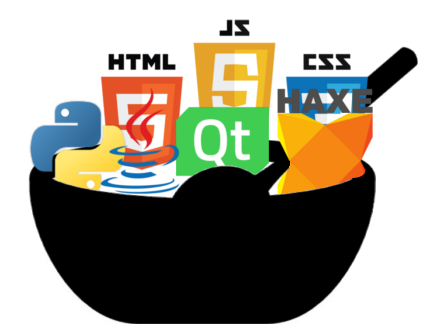
\includegraphics[width=0.5\textwidth]{./figures/techsoup.png}
		\caption{Some cross-platform technologies}
		\label{F:tech-soup}
	\end{center}
\end{figure}


More than twenty years putting effort to solve this problem has created a 
technological soup (Figure \ref{F:tech-soup}). Qt, Python, JavaScript, Java and 
Haxe
\cite{qt-web}\cite{py-web}\cite{js-wiki}\cite{what-is-java}\cite{what-is-haxe}
are some examples among many others.

\subsection{Qt}

Qt is a complete cross-platform software framework with ready-made UI elements,
\CC libraries, and a complete integrated development environment with tools for 
everything you need to develop software for any project \cite{qt-web}.

\begin{codefigure}
	\cppexternal[
		caption=Qt hello world,
		label=L:qt-hello-world,
		%
		classoffset=1,
		morekeywords={QPushButton, QApplication}
	]{source/qt_hello_world.cpp}
\end{codefigure}

Code of Listing \ref{L:qt-hello-world} creates a window and add a button that
says Hello World with size 100x30.

\subsection{Python}

Python is an example of a scripting programming language. The main design rule
was to be very easy to read. For this reason, Python is the only language where
tabulation rules must be strictly followed to make the program work.

It is also considered an object-oriented language suitable for many purposes.
It has a clear, intuitive syntax, powerful high-level data structures, and a
flexible dynamic type system \cite{An93pythonfor}.

Python is often used to create terminal programs or web services because GUI
are not supported by default, but there are many frameworks that can be used,
for instance, \textbf{Kivy}.

\begin{codefigure}
	\pythonexternal[
		caption=Kivy hello world,
		label=L:kivy-hello-world,
	]{source/kivy_hello_world.py}
\end{codefigure}

As Listing \ref{L:kivy-hello-world} shows up, a window with is created with a
button which text is "Hello World".

\subsection{JavaScript}

JavaScript is also a well-know widely-used scripting programming language. It is commonly used
alongside with HTML and CSS as core technologies to make webpages. Moreover, due
to its flexibility, it is used in many other fields like game programming or
desktop applications.

It has many interpreters but all of them has to fulfill ECMAScript
specification. V8 is an example of JavaScript engine used in Google Chrome and
Node.js \cite{nodejs-web}. This latter example is widely used to build terminal
applications and web services.

Some years ago, developing trends were to create web applications instead of
desktop ones since it has less development cost and all platforms have browsers
indeed. For this reason, web technologies have grown a lot and today can be
compared with desktop technologies.

But web applications have several technological problems. The main one is that
since the code is download from an external non-trusted source, the browser
must limit the access to the computer for security reasons
\cite{securing-your-browser}. For instance, web applications can not read the
user's file system. Moreover, programs have higher load periods due to those
downloads.

Another important fact is that user experience (UX) will never be as good as
using a desktop application due to it is embedded inside the browser and some
space is lost due to menus.

% TODO: *** what about chrome/chromium apps, is it the same?***
% Respuesta: Realmente lo problematico es que el JavaScript del browser
% es mas limitado.

\subsubsection{Electron}

Electron is a Node.js framework that lets developers build cross-platform
desktop applications using JavaScript, HTML, and CSS \cite{electron-web}. As
seen before, web technologies are now able to race desktop ones in terms of
performance and scalability.

The idea behind Electron is take profit of the fact that Node.js and Chrome uses
the same JavaScript engine (V8) to let Node.js instantiate Chrome windows and
use them as user interface. Moreover, Electron Chrome windows are able to use
all extra Node.js modules, for instance, to be able to access the computer's
file system.

UX is improved respect web pages because Chrome menus are removed and
application code is now inside user's computer.

For short, Electron help developers to create cross-platform desktop 
applications using the same technologies that the ones used to create a webpage.

\subsubsection{NW.js}

NW.js, previously known as node-webkit, works on the contrary of Electron. It
is just a Chrome web browser where you can call all the node modules
\cite{nwjs-web}. So the main difference is the entry point of the application.
In Electron, the start point of your program execution is Node.js while on
NW.js the entry point is an HTML file.

\subsection{Java}

This well-known programming language is one of the most used to build
cross-platform desktop applications due to its maturity. Java is a
general-purpose, concurrent, class-based, object-oriented language and it is
designed to be easy to learn in order to let many programmers to have fluency
in the language \cite{java-8-specs}.

Classic compiled languages, such as, C and \CC, directly compile into machine
code, which is directly interpreted by the hardware. As opposed to C and \CC,
Java can be considered a virtual machine programming language.

\begin{codefigure}
	\javaexternal[
	caption=Java hello world,
	label=L:java-hello-world,
	%
	classoffset=1,
	morekeywords={HelloWorldApp}
	]{source/HelloWorldApp.java}
\end{codefigure}

Listing \ref{L:java-hello-world} is an example of Java program that prints the
test “Hello World!” into the terminal. All files must contain just one class and
the name of the file must match. The static function called main is the entry
point of the application and in this example uses the standard output to print
a message.

\subsection{Haxe}

Finally, Haxe is a high-level open source programming language that can be 
transcompiled many other languages. It has an ECMAScript-oriented syntax but 
with the peculiarity that can be typed \cite{what-is-haxe}. 

\begin{table}[htb]
\begin{center}
\begin{tabular}{|l|l|l|}
\hline
{\bf Name }		& {\bf Output Type} & {\bf Main usages}  \\ \hline \hline
JavaScript		& Sourcecode		& Browser, Desktop, Mobile, Server \\ \hline
Neko			& Bytecode			& Desktop, Server   \\ \hline
PHP				& Sourcecode		& Server   \\ \hline
Python			& Sourcecode		& Desktop, Server   \\ \hline
\CC				& Sourcecode		& Desktop, Mobile, Server   \\ \hline
ActionScript 3	& Sourcecode		& Browser, Desktop, Mobile   \\ \hline
Flash			& Bytecode			& Browser, Desktop, Mobile   \\ \hline
Java			& Sourcecode		& Desktop, Server   \\ \hline
C\#				& Sourcecode		& Desktop, Mobile, Server   \\ \hline
\end{tabular}
\caption{Haxe use cases \cite{what-is-haxe}}
\label{T:haxe-use-cases}
\end{center}
\end{table}

Table \ref{T:haxe-use-cases} shows up many languages in which Haxe can be
compiled. Then lets see a bit of Haxe syntax.

\begin{codefigure}
	\haxeexternal[
		caption=Haxe hello world,
		label=L:haxe-hello-world,
		%
		classoffset=1,
		morekeywords={Main}
	]{source/Main.hx}
\end{codefigure}

As we can see in Listing \ref{L:haxe-hello-world}, Haxe can be typed defining 
variables that way: \haxeinline{var text: String}. This code can be compiled
for example to Python other languages using the terminal command:

\begin{terminal}[caption=Haxe python transcompilation command, label=haxe-2-py]
%
\terminalcmd[haxe -main Main.hx -python main.py]
%
%\terminalcmd%

\end{terminal}

\section{Electron}
\label{S:electron}

The technology that fits better with the project's specifications is Electron. 
There are several projects like this one that are developed using this 
framework. Even it is probably not as mature as other ones, it had a big impact 
in the developers community. Figure \ref{F:electron-applications} shows several
applications developed using Electron \cite{electron-web}.

\begin{figure}[htb]
	\begin{center}
		\begin{subfigmatrix}{4}
			\subfigure[Visual Studio Code (Microsoft)]
			{
\includegraphics{./figures/vs-code-icon.png}\label{SF:S1}} 
			\subfigure[Atom]
			{
\includegraphics{./figures/atom-icon.png}\label{SF:S1}} 
			\subfigure[Github Desktop]
			{
\includegraphics{./figures/github-desktop-icon.png}\label{SF:S1}} 
			\subfigure[Slack]
			{
\includegraphics{./figures/slack-icon.png}\label{SF:S1}} 
		\end{subfigmatrix}
		\caption{Electron application examples}
		\label{F:electron-applications}
	\end{center}
\end{figure}

Moreover, the development of web applications has been evolved very fast with
the objective to have complex programs with a very good scalability and without
putting so much effort.

Then, some examples show how Electron works in a little more of detail.
Complete code is available on Appendix \ref{APP:electron-hello-world}.

\subsection{Main process}

% TODO: NO ENTIENDO EL COMOR?! jajaja
% JavaScript solo tiene un tread pero puedes tener muchos procesos en paralelo
% para hacer cosas a la vez. Osea:
%    - En C y Java puedes utilizar semaforos para acceder a memoria comparida.
%    - En javascript tienes que utilizar mecanismos de comunicacion como si
%      fueran aplicaciones diferentes.
% Otra cosa seria que desde un lenguaje multithreaded lances varios threads 
% corriendo javascript o que un modulo javascript hecho en C aplique 
% multithread.

JavaScript is a single threaded programming language. In order to be able to
work in parallel, Electron has several processes. The initial one is called 
main process. It is in charge of create all browser windows, communicate them,
to build application menus and control context events.

\begin{codefigure}
	\jsexternal[
		caption=Electron app events,
		label=L:electron-app-events
	]{source/electron-app.js}
\end{codefigure}

Code of Listing \ref{L:electron-app-events} is an example of the most common
handled events. The most important is the \textit{"ready"} event, where the
main window of the application is created.

\subsection{Browser window}

Once event \textit{"ready"} is called, browser windows can be created. Each
window has its own independent process called renderer. The way to create
windows is shown on Listing \ref{L:electron-create-window}.

\begin{codefigure}
	\jsexternal[
		caption=Electron window creation,
		label=L:electron-create-window,
	]{source/electron-create-window.js}
\end{codefigure}

Browser windows can be created using several parameters to define its initial
behavior, for instance: width, height, position, etc. They can load files  
using several protocols (HTTP, FTP, etc) or directly access to local hard disk.
In Electron, the most common way is to use local files to reduce load time and
let the application work without Internet connection. Finally, window objects
also have events, for example: \textit{"closed"}, \textit{"ready-to-show"},
\textit{"move"}\dots

\subsection{Interprocess communication}

Finally, to be able to communicate the main process and the renderer processes, 
Electron provides inter-process communication (IPC). By default, it can provide
communications main-to-renderer and renderer-to-main. Therefore, if
renderer-to-renderer communication is needed, a bridge must be implemented
inside the main process.

% TODO: Pongo ejemplo de codigo de esto tambien? 
% TODO: dependiendo del número final de páginas

\section{Web technologies}

Core World Wide Web technologies, as seen before, are JavaScript, HTML and CSS.
Nevertheless, there are many other specialized tools to solve specific deficits 
those technologies have. For instance, Typescript, SCSS and Gulp are used to
enhance scalability and maintainability. 

\subsection{Typescript}

Typescript\cite{typescript-web} is a programming language created by Microsoft
that is a typed superset of JavaScript that compiles to plain JavaScript. It has
two main advantages:

\begin{description}
	\item[Typed language]
	Since Typescript is a typed language and it has a compilation process, any
	mismatch of parameters used in a function call are detected before testing
	anything. Also, Integrated Development Environments (IDEs) can help
	developers highlight those mismatches because type information is provided.
	
	\item[Compiles to plain Javascript]
	There are many web browsers and not all of them support current ECMAScript 
	standard. Using TypeScript developers don't need to take care of it because
	target JavaScript version can be selected.

\end{description}

Many JavaScript libraries also provide its TypeScript typings. Using this 
information, the compiler can detect if the library is properly used.

\begin{codefigure}
	\tsexternal[
		caption=TypeScript example,
		label=L:typescript-example,
		%
		classoffset=1,
		morekeywords={Person, T, GreetingsCallback, Greetings}
	]{source/hello-world.ts}
\end{codefigure}

Listing \ref{L:typescript-example} is a TypeScript example that shows some
advanced type declarations. As can be seen, it supports templates, interfaces
and even defining function types.

Each time TypeScript is compiled, a tool called TsLint can be used to check if 
some programming style guides are followed. Follow this rules, even if it is 
not strongly needed, is very useful to keep code easy-to-read. For instance, 
a common rule used in JavaScript is to name variables following lower camel case
and upper camel case for classes.

\subsection{Sass}

Like TypeScript, SASS is a code transcompiler, but it translates from SASS to
CSS. It is designed to improve CSS functionalities.

\begin{codefigure}
	\sassexternal[
		caption=Sass example,
		label=L:sass-example,
		%
		classoffset=2,
		morekeywords={\$app_green, flex-row}
	]{source/example.scss}
\end{codefigure}

Listing \ref{L:sass-example} helps to see all the advantages that SASS provides.
The main ones are:

\begin{description}
	\item[Nesting CSS selectors]
	Improves code scalability. 

	\item[Variables]
	Helps to define palettes, sizes, etc.
	
	\item[Mixins]
	Similar to functions, they are very useful to define common behaviors.
	
\end{description}

\subsection{Gulp}

Gulp is a toolkit for automating painful or time-consuming tasks in your
development workflow, so you can stop messing around and build something
\cite{gulp-web}.

This project has several routine tasks, such as launch electron, compile
TypeScript and SASS each time a file change happens, etc. For this reason, 
several gulp tasks are created to help development.

\begin{codefigure}
	\jsexternal[
		caption=Gulp task to compile SASS,
		label=L:gulp-sass,
	]{source/gulp-sass.js}
\end{codefigure}

For instance, Listing \ref{L:gulp-sass} shows how a task to compile all .sass 
files is implemented.

% \chapter{Software architecture}
\label{S:architecture}

% TODO: En este apartado empiezo a poner diagramas, los pongo a color o
% mejor en blanco y negro??
% TODO: a color (no creo que tengamos que imprimir)

“Most systems work better they are kept simple rather than complicated”
\cite{kiss-wiki}. This is the main statement of the KISS principle, acronym for
“Keep it simple, stupid”. KISS philosophy is very used on software development
because code tends to chaos and disorder. If the implementation of a
functionality is not properly thought, it adds complexity to the program work
flow. Therefore, to reduce the architecture entropy should be one of the main
design patterns on any software.

Model-View-Controller (MVC) is a well-known software architecture that consists
on the use of this tree elements to build a user interface. It was introduced 
by Trygve Reenskaug in the seventies \cite{mvc-past-present}. When web
applications appeared, this model was applied in many important projects
like \href{https://support.microsoft.com}{Microsoft Support}. 

% TODO: NO SE COMO PONER UNA WEB COMO EJEMPLO: como cita o hipervinculo??
% TODO: como cita.

\begin{figure}[htb]
	\begin{center}
		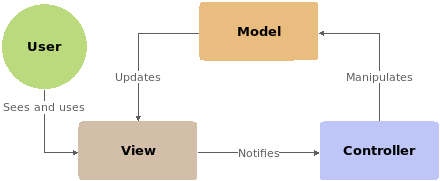
\includegraphics[width=0.5\textwidth]{./figures/mvc.png}
		\caption{Diagram of interactions within the MVC pattern.
				 \cite{mvc-wiki}}
		\label{F:mvc}
	\end{center}
\end{figure}

As shown on Figure \ref{F:mvc}, it is a simple model to represent a user
interface (UI). What user sees is represented by the view. Each time the user 
performs an action, view notifies the controller and it modifies the current
model. Since view is watching changes on the model, this change is detected and,
thus, view is affected.

The problem is that this architecture becomes complex and complex while 
increasing the number of views. Actions from a view can affect other views'
model and this changes can trigger other actions. This complexity could even
generate unexpected loops as Figure \ref{F:mvc-complex} proves.

\begin{figure}[htb]
	\begin{center}
		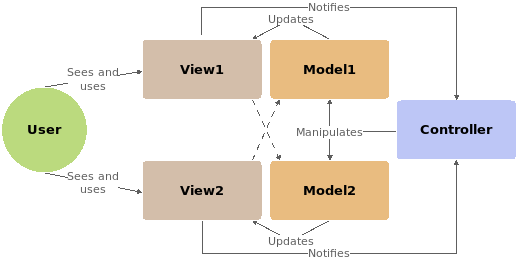
\includegraphics[width=0.6\textwidth]{./figures/mvc-complex.png}
		\caption{Diagram of interactions within the MVC pattern with many views}
		\label{F:mvc-complex}
	\end{center}
\end{figure}

\section{Flux architecture}

In order to solve the MVC scalability problem, Facebook launched Flux, represented
on Figure \ref{F:flux}. Now views are watching a plain object (state) saved
inside the store. Actions are also plain objects that are dispatched changing
the current stored state.

\begin{figure}[htb]
	\begin{center}
		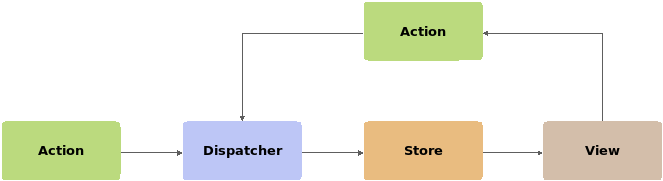
\includegraphics[width=0.7\textwidth]{./figures/flux.png}
		\caption{Diagram of Flux}
		\label{F:flux}
	\end{center}
\end{figure}

Even through views just wait change events produced by the store and render
themselves using the current state information. Note that the render processes
must not call any action.

\section{React}

React is an implementation of the Flux view block. It is a component-based 
JavaScript library to build user interfaces \cite{react-web}. Each React
component can have input properties, state, and must implement a render
function. Moreover, to make things easier, React supports JSX which are
JavaScript files where HTML code can be directly used.

\begin{codefigure}
	\jsxexternal[
		caption=React hello world,
		label=L:react-hello-world,
		%
		classoffset=1,
		morekeywords={HelloMessage, React, Component, ReactDOM},
		classoffset=2,
		morekeywords={<HelloMessage},
	]{source/react-hello-world.jsx}
\end{codefigure}

Listing \ref{L:react-hello-world} shows up an example of React component. It is
stateless, it has a property call name and an easy render function to create a
\textit{div} with text. Render functions can also have components inside
themselves. That way, React creates a component tree \ref{F:react-tree}.

\begin{figure}[htb]
	\begin{center}
		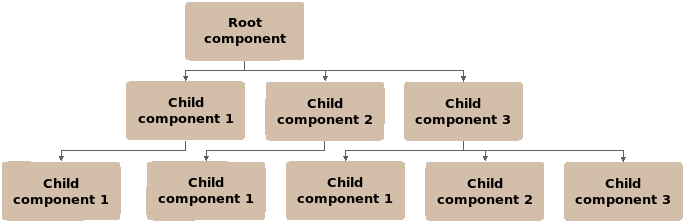
\includegraphics[width=0.7\textwidth]{./figures/react-tree.png}
		\caption{React tree}
		\label{F:react-tree}
	\end{center}
\end{figure}

Components may need to perform actions. Those cannot be performed on render 
function, as seen before. Instead, to do that each component have a lifecyle.
It consists of a set of functions that are triggered when some external events
happen. Most used ones are \textit{"componentWillMount"} and 
\textit{"componentWillUnmount"}. Components also can listen to its view
events, for instance button clicks, to perform actions.

\section{Redux}

Redux was inspired by several important qualities of Flux. Like Flux, Redux
prescribes that the model update logic is concentrated in a certain layer of
the application (“stores” in Flux, “reducers” in Redux) \cite{redux-prior-art}.
Redux have tree principles must be followed \cite{redux-principles}.

\begin{description}
	\item [Single source of truth]
	The state can be stored easily if just one store is used. Furthermore, the
	application will be easy to debug. Once again, keep it simple.
	
	\item [State is read-only]
	The only way to update the state is using actions. Each time the state
	changes, a new independent state must be created.

	\item [Changes are made with pure functions]
	Reducers must be pure functions, that results in the following statement:
	"using the same initial state, repeating the same list of actions must
	produce the same final state".

\end{description}

\begin{figure}[htb]
	\begin{center}
		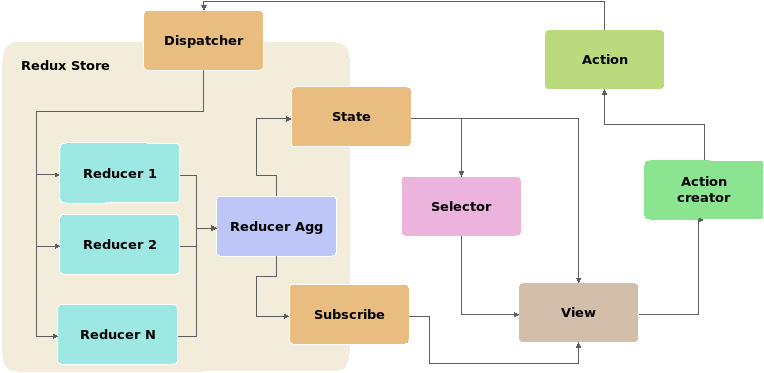
\includegraphics[width=0.8\textwidth]{./figures/redux.png}
		\caption{Redux architecture}
		\label{F:redux-architecture}
	\end{center}
\end{figure}

Figure \ref{F:redux-architecture} shows up the overall Redux's architecture.
First of all, a store must be created. This store contains reducers that map
action, created by action creators, into state changes. If needed, selectors
can be used to cache some state costly transformations. Store also lets 
to subscribe to state change notifications.

\subsection{Action creators}

An action is a plain JavaScript object that contains a field called type to 
identify it and other optional fields. Same type of action can be created in
many places so it is extremely recommended to use action creators.

Action creators are functions that create those objects. Normally are defined
using lambdas. An example of action creator is shown on Listing
\ref{L:redux-action-creator}. This one is intended to create an action that
appends a text item into the state.

\begin{codefigure}
	\jsexternal[
		caption=Redux action creator,
		label=L:redux-action-creator,
	]{source/redux-action-creator.js}
\end{codefigure}

\subsection{Reducers}

Reducers aim to return new states each time an action is produced. They must be
implemented using pure functions. A function must follow tree statements to be 
considered pure.

The fist one is \textbf{mapping}. To fulfill it means that same input always 
results on the same output. Therefore, pure functions can not generate random
numbers, current date, nor depend on external variables. If this statement is
not followed, functions are difficult to test since its return value is
unpredictable. To make a function fulfill mapping is as easy as adding 
unpredictable values as parameters. Listing \ref{L:mapping-example} is an 
example of function that multiplies a random value with a parameter.

\begin{codefigure}
	\jsexternal[
	caption=Mapping example,
	label=L:mapping-example,
	]{source/mapping.js}
\end{codefigure}

The second statement is \textbf{avoid side effects}. This means that functions
must not modify anything outside them. If a pure function needs to access
outside, maybe it is ill-designed. 

\begin{codefigure}
	\jsexternal[
	caption=Avoid side effects example,
	label=L:side-effects-example,
	]{source/no-side-effects.js}
\end{codefigure}

The last one is \textbf{no external mutable}. This means that the output of a
function must be independent to changes other variables. But how can this
happen? Easy, when a JavaScript object is assigned to another variable, it is a
reference of the first one, not a copy. If any of both variables changes, it
will affect also to the other. A simple example of this issue is shown on 
Listing \ref{L:obj-ref}.

\begin{codefigure}
	\jsexternal[
		caption=Object reference effect,
		label=L:obj-ref,
	]{source/obj-ref.js}
\end{codefigure}

Therefore, an example of non pure function due to no external mutation is to
return an object parameter. In order to follow no external mutable principle,
the returned object must be a copy of the one provided as parameter (Figure
\ref{L:no-external-mutation}).

\begin{codefigure}
	\jsexternal[
	caption=No external mutation example,
	label=L:no-external-mutation,
	]{source/no-external-mutation.js}
\end{codefigure}

Then, applying this three principles, Listing \ref{L:redux-reducer} shows up an
example of reducer for the action created on Listing 
\ref{L:redux-action-creator}.

\begin{codefigure}
	\jsexternal[
		caption=Redux reducer,
		label=L:redux-reducer,
	]{source/redux-reducer.js}
\end{codefigure}

This function is called by the store each time an action is dispatched. 
Reducers can be aggregated using a function provided by Redux called
\textit{"combineReducers"}. Listing \ref{L:redux-agg-reducers} shows an example.

\begin{codefigure}
	\jsexternal[
		caption=Reducer aggregation,
		label=L:redux-agg-reducers,
	]{source/redux-agg-reducers.js}
\end{codefigure}

\subsection{Selectors}
\label{S:selectors}

Selectors are functions that can cache the return value and it is just 
recomputed if any of the input parameters changes. For instance, a selector
can be created to select items that starts with letter 'I'. This example is
shown on Listing \ref{L:redux-selector}.

\begin{codefigure}
	\jsexternal[
		caption=Redux selector,
		label=L:redux-selector,
	]{source/redux-selector.js}
\end{codefigure}

\subsection{Store}

Creating a store is as easy as providing the root reducer and the initial state.
Then actions can be dispatched and a function can be subscribed to detect any
state change.

Listing \ref{L:redux-store} shows how to create a store. Selector created in
Section \ref{S:selectors} is used to compute a subset of items just if the
item list has change. Also, several actions are dispatched.

\begin{codefigure}
	\jsexternal[
		caption=Redux store creation and management,
		label=L:redux-store,
	]{source/redux-store.js}
\end{codefigure}

\section{Action observables}

Observables are data streams provided by a library called Reactive Extensions
for JavaScript (rxjs). The idea is to treat those streams as asynchronous 
events and apply fluent query operators to describe behaviors.

\begin{codefigure}
	\jsexternal[
		caption=Rxjs observable to count seconds until last click,
		label=L:rxjs-simple-observable,
	]{source/rxjs-simple-observable.js}
\end{codefigure}

As shown on Listing \ref{L:rxjs-simple-observable}, complex behaviors can be
implemented in an easy to read way using this library. The example shows up
how to count the difference in time between two button clicks. To do that, 
an observable is created to watch the event click of a button. The operator scan
caches the last returned value sending it as first parameter of the callback
function. Last scanned is mapped to get the difference in seconds of last
and current time values. Finally, this difference is printed on a text element.

Since Redux's reducers must be pure functions and there are many complex
behaviors that have to be chained when some actions are produced, Redux
Observables provide a middleware that handles action streams using rxjs
observables. The observable is executed after the action has been reduced.
So Redux architecture (Figure \ref{F:redux-architecture}) must be complemented 
with Figure \ref{F:redux-observables-architecture}.

\begin{figure}[htb]
	\begin{center}
		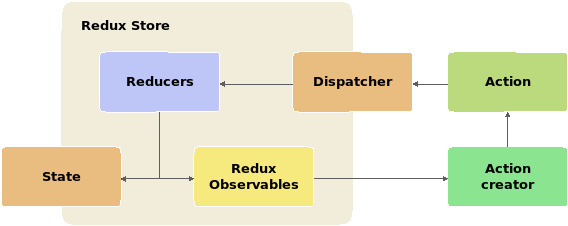
\includegraphics[width=0.6\textwidth]{./figures/redux-observables.png}
		\caption{Redux Observables architecture}
		\label{F:redux-observables-architecture}
	\end{center}
\end{figure}

\section{React-Redux}

To let React and Redux work together, Redux store must be provided to whole
React tree. Also, action creators and state have to be mapped into React
properties.

A package called react-redux adds a React component named \textit{"Provider"}
that inserts a store inside the React tree. Children of \textit{"Provider"} can
connect to it by using the \textit{"connect"} function. It needs two 
parameters, one to map the store state to component's properties and a second 
one to map actions.

\begin{landscape}
\begin{figure}[htp]
	\begin{center}
		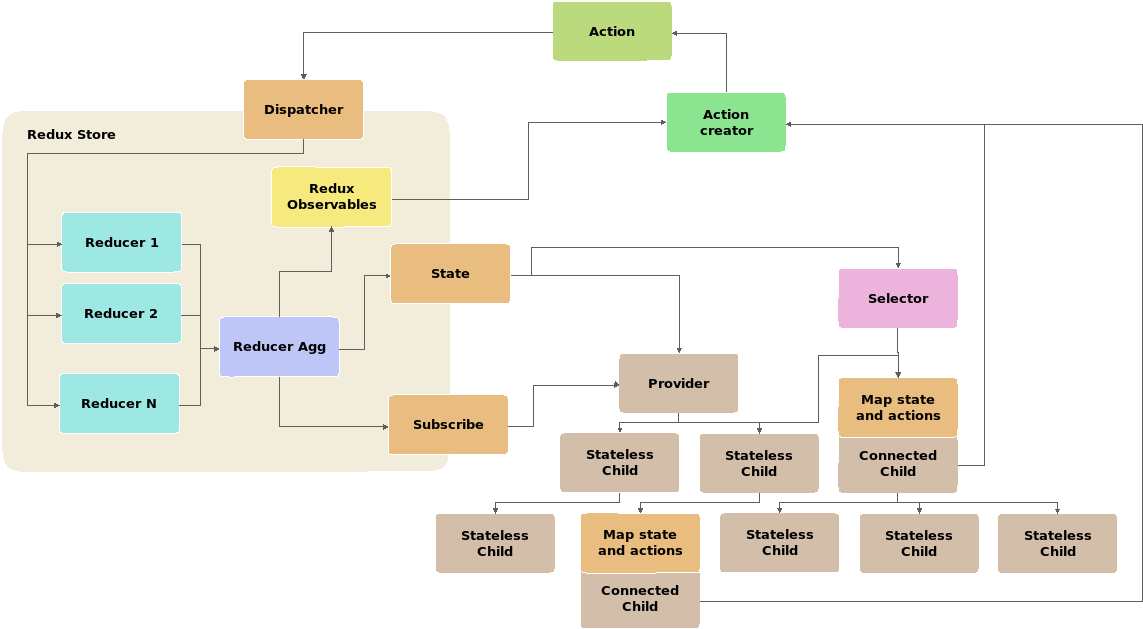
\includegraphics[width=1.3\textwidth]
		{./figures/overall-architecture.png}

		\caption{Overall architecture}
		\label{F:overall-architecture}
	\end{center}
\end{figure}
\end{landscape}






\texttt{\chapter{Digital forensics analysis}
\label{S:df-analysis}}

The Sleuth Kit (TSK) is an open source cross-platform collection of terminal
applications and a C library that allows investigators to analyze disk images
and recover files from them \cite{tsk-web}. It is divided in file system and
volume tools. 

The first group allows investigators to examine the file system of a suspect
computer in a non-intrusive way. Main file system tools are shown on Table
\ref{T:tsk-fs-tools}.

\begin{table}[htb]
\begin{center}
\begin{tabular}{|l|l|l|}
\hline
{\bf Command }	& {\bf Description }  \\ \hline \hline
fsstat & Shows file system details and statistics \\ \hline \hline
fls	& Lists allocated and deleted file names in a directory \\ \hline
ffind & Finds allocated and unallocated file names \\ \hline \hline
icat & Extracts the data units of a file \\ \hline
\end{tabular}
\caption{Main file system tools from TSK \cite{tsk-tools-wiki}}
\label{T:tsk-fs-tools}
\end{center}
\end{table}

Volume tools are the ones that brings off the layout of disks and another media.
They are needed to identify where partitions are located to be able to proceed
with a file system analysis. Table \ref{T:tsk-v-tools} lists main volume tools.

\begin{table}[htb]
\begin{center}
\begin{tabular}{|l|l|l|}
\hline
{\bf Command }	& {\bf Description }  \\ \hline \hline
mmls & Displays the layout of a disk \\ \hline \hline
mmstat & Display details about a volume system \\ \hline
\end{tabular}
\caption{Main volume tools from TSK \cite{tsk-tools-wiki}}
\label{T:tsk-v-tools}
\end{center}
\end{table}

In order to explain how The Sleuth Kit works easily, an example will be used.
In that specific case, an investigator will extract the timeline for an image
and will look for a file called \textit{letter.txt} to print its content.

\section{The Sleuth Kit analysis}
\label{S:tsk-analysis}

To start the TSK analysis, the command \textit{mmls} is used to output the 
information of all partitions. If volume type is not specified, TSK will
autodetect it. The output will look like Listing \ref{L:tsk-mmls-output}.
This example has tree volumes:

\begin{description}
	\item [Primary Table (\#0)]
	It contains the primary table. 
	
	\item [Unallocated]
	Unallocated space.

	\item [Win95 FAT32 (0x0C)]
	This partition has an offset of 56 sectors and it contains a file system formatted with FAT32.
	
\end{description}

\begin{terminal}[caption=TSK mmls output example, label=L:tsk-mmls-output]
	%
	\terminalcmd[mmls hdd-001.dd]
	%
	DOS Partition Table
	Offset Sector: 0
	Units are in 512-byte sectors
	
	Slot         Start        End          Length       Description
	00:  Meta    0000000000   0000000000   0000000001   Primary Table (#0)
	01:  -----   0000000000   0000000055   0000000056   Unallocated
	02:  00:00   0000000056   0007925759   0007925704   Win95 FAT32 (0x0C)
	%\terminalcmd%
\end{terminal}

To perform a deeper analysis, file system tools must be used. In that case,
those will need the offset of 56 sectors to be specified. The  first tool,
\textit{fsstat}, will display some file system characteristics, for instance,
root inode, sector size and the file system layout.

Also, the registers inside the disk can be listed in a non-intrusive way using 
\textit{fls}. In this specific example (Listing \ref{L:fls-output-example}),
the file system contains four folders. One of them,  
\textit{\_NTITL\textasciitilde1} is deleted. Also, some virtual registers are
displayed (\$MBR, \$FAT1, \$FAT2, \$OrphanFiles). If it is necessary to go
through the file system tree, a directory inode can be specified to list
registers inside it or analyze whole disk recursively.

\begin{terminal}[caption=TSK fls output example,label=L:fls-output-example]
%
\terminalcmd[fls -o 56 hdd-001.dd]
%
d/d 4:	.Trash-1000
d/d * 5:	_NTITL~1
d/d 7:	Personal
d/d 9:	Imagenes
v/v 126563459:	$MBR
v/v 126563460:	$FAT1
v/v 126563461:	$FAT2
d/d 126563462:	$OrphanFiles
%\terminalcmd%
\end{terminal}

Several times, it is necessary to export the whole file system in order to obtain
processed information using other tools. The command arguments that are
necessary are:

\begin{terminal}[caption=Export file system to CSV,label=L:fls-csv-export]
%
\terminalcmd[fls -m / -o 56 -r hdd-001.dd > fs.csv]
%
%\terminalcmd%

\end{terminal}

This CSV file can also be used to generate timelines using a specific TSK tool 
called \textit{mactime}. The output format of \textit{mactime} can be also
adjusted to process it with any CSV program. Columns shown on Listing
\ref{L:tsk-timeline} are: date, file size, activity type, Unix permission, User
\& Group IDs, inode and file name. Allowed activity types are: modified (m),
accessed (a), changed (c) and created (b).

\begin{terminal}[caption=Haxe python transcompilation command, label=L:tsk-timeline]
%
\terminalcmd[haxe -main Main.hx -python main.py]
%
Xxx Xxx 00 0000 00:00:00   338558 ..c. r/rrwxrwxrwx 0        0        10758    /Imagenes/bufon.png
         10 ..c. r/rrwxrwxrwx 0        0        10889    /Personal/file.txt
       4096 ..c. d/drwxrwxrwx 0        0        11142    /.Trash-1000/info
       4096 ..c. d/drwxrwxrwx 0        0        11144    /.Trash-1000/files
         70 ..c. r/rrwxrwxrwx 0        0        11274    /.Trash-1000/info/carta.txt.trashinfo
         72 ..c. r/rrwxrwxrwx 0        0        11401    /.Trash-1000/files/carta.txt
       4096 ..c. d/drwxrwxrwx 0        0        4        /.Trash-1000
          0 ..c. d/drwxrwxrwx 0        0        5        /_NTITL~1 (deleted)
       4096 ..c. d/drwxrwxrwx 0        0        7        /Personal
       4096 ..c. d/drwxrwxrwx 0        0        9        /Imagenes
Fri Aug 25 2017 00:00:00   338558 .a.. r/rrwxrwxrwx 0        0        10758    /Imagenes/bufon.png
         10 .a.. r/rrwxrwxrwx 0        0        10889    /Personal/file.txt
       4096 .a.. d/drwxrwxrwx 0        0        11142    /.Trash-1000/info
       4096 .a.. d/drwxrwxrwx 0        0        11144    /.Trash-1000/files
         70 .a.. r/rrwxrwxrwx 0        0        11274    /.Trash-1000/info/letter.txt.trashinfo
         72 .a.. r/rrwxrwxrwx 0        0        11401    /.Trash-1000/files/letter.txt
       4096 .a.. d/drwxrwxrwx 0        0        4        /.Trash-1000
          0 .a.. d/drwxrwxrwx 0        0        5        /_NTITL~1 (deleted)
       4096 .a.. d/drwxrwxrwx 0        0        7        /Personal
       4096 .a.. d/drwxrwxrwx 0        0        9        /Imagenes
Fri Aug 25 2017 15:06:56   338558 m..b r/rrwxrwxrwx 0        0        10758    /Imagenes/bufon.png
Fri Aug 25 2017 15:07:18     4096 m..b d/drwxrwxrwx 0        0        9        /Imagenes
Fri Aug 25 2017 15:07:22        0 m..b d/drwxrwxrwx 0        0        5        /_NTITL~1 (deleted)
Fri Aug 25 2017 15:07:30     4096 m..b d/drwxrwxrwx 0        0        4        /.Trash-1000
Fri Aug 25 2017 15:08:04       72 m..b r/rrwxrwxrwx 0        0        11401    /.Trash-1000/files/carta.txt
Fri Aug 25 2017 15:08:06       70 m..b r/rrwxrwxrwx 0        0        11274    /.Trash-1000/info/carta.txt.trashinfo
Fri Aug 25 2017 15:08:12     4096 m..b d/drwxrwxrwx 0        0        11142    /.Trash-1000/info
< 4096 m..b d/drwxrwxrwx 0        0        11144    /.Trash-1000/files
Fri Aug 25 2017 15:08:22       10 m..b r/rrwxrwxrwx 0        0        10889    /Personal/file.txt
       4096 m..b d/drwxrwxrwx 0        0        7        /Personal
%\terminalcmd%

\end{terminal}

As Listing \ref{L:tsk-timeline} shows, the inode 11401 contains a file called
letter.txt. Print its content can be easily done using the command
\textit{icat}. 


\begin{terminal}[caption=Export a file contained inside the file system,label=L:icat-export]
%
\terminalcmd[icat -o 56 hdd-001.dd 11401]
%
Mr. Someone,
You must know I am guilty!

Best regards,
Nobody Jones
%\terminalcmd%

\end{terminal}


\section{The Sleuth Kit JavaScript}

% TODO:
% Quiero dar enfasis en que esto es parte del desarrollo del proyecto y no se 
% si esta bien hecho asi...

Bearing in mind the need to develop a wrapper to connect TSK with a JavaScript
application \textbf{The Sleuth Kit JavaScript (TSK-js) has been created}. This
wrapper must be able to execute the same analysis carried out in the previous chapter
(Chapter \ref{S:tsk-analysis}) but using JavaScript.

It has been raised to create a JavaScript object with one construction argument
in with the image file path is specified. This object will have the necessary
methods to perform the entire analysis. Those methods are explained on Table
\ref{T:tsk-js-object-methods}.

\begin{table}[htb]
\begin{center}
\begin{tabular}{|l|l|l|}
\hline
{\bf Method }	& {\bf Arguments} & {\bf Returns } \\ \hline \hline
Analyze	& None & Type (disk/partition) and if type disk, returns\\
& 	   & its partitions specifying the offset sectors \\ \hline
List & Offset sectors and inode & List file system files \\ \hline
Get & Offset sectors and inode & Buffer with inode content \\ \hline
Timeline & Offset sectors, inode & Timeline results \\ 
& and callback function & \\ \hline
Search & Needle, offset sectors, & None \\ 
& inode and callback function & \\ \hline
\end{tabular}
\caption{TSK-js object methods}
\label{T:tsk-js-object-methods}
\end{center}
\end{table}

Search and Timeline take some time to execute. That is why both have a callback
function as parameter. Each time a result is found, this callback function is
called.

An example of JavaScript code that can perform the analysis proposed on 
Chapter \ref{S:tsk-analysis} is shown of Listing \ref{L:tsk-js-analysis}.

\begin{codefigure}
	\jsexternal[
		caption=The Sleuth Kit JavaScript analysis,
		label=L:tsk-js-analysis,
		%
		classoffset=1,
		morekeywords={TSK},
	]{source/tsk-js-analysis.js}
\end{codefigure}

This analysis can be executed using the following command:

\begin{terminal}[caption=Execute The Sleuth Kit JavaScript analysis
,label=L:tsk-js-execute-analysis]
%
\terminalcmd[node analysis.js hdd-001.dd]
%
File found!
Print it's content:
---------------------------
Mr. Someone,
You must know I am guilty!

Best regards,
Nobody Jones
---------------------------
Timeline length '29'
%\terminalcmd%

\end{terminal}

The implementation of this package is done using \CC and node-gyp that is a 
compiler to create Node.js addons \cite{node-gyp-github}.

A TypeScript types file is provided in order to help transcompiler with type 
validations. Typings can be found on Appendix \ref{APP:tsk-js-typings}.
This package is available on Node Package Manager
(\url{https://www.npmjs.com/package/tsk-js}). The source code is also available
on GitHub (\url{https://github.com/FRG-UPC-Deliverables/tsk-js}).


% \chapter{Img-spy}
\label{S:img-spy}

Imgspy is GUI (graphic user interface) that performs digital forensic analysis
using the sleuthkit as library. It is coded using Typescript for the logic,
HTML5 to define the view and Sass the look and feel. Javascript and CSS are not 
directly used because Typescript increases the code reliability since types 
can be defined while Sass adds flexibility to the style definition, such as, functions and inheritance.

The source code of the project is within the \textit{src} folder. Typescript
and Sass need to be compiled because they cannot be directly interpreted. For
this reason, \textit{dist} folder contains all the source code changing the 
Typescript files for Javascript ones and Sass for CSS.

The application is divided in a frontend and a backend. The last one is 
responsible of the costly operations and the window management, while frontend
shows the user interface.

\begin{description}
	\item[main] Typescript files of the backend.
	\item[app] Typescript and HTML files of the frontend. They contain the view
	and the application logic.
	\item[lib] Javascript libraries not uploaded to npm.
	\item[i18n] Internationalization files.
	\item[style] Sass files. They contain the look and fell of the application.
\end{description}

%%% RESUMEN DE COMO FUNCIONA EL BACKEND

Electron starts a process called Main which loads a Node.js script. It is in
charge of manage the whole application. This process launches two instances, the
WindowManager and the FileSystemWorkersManager.

The WindowManager creates all windows shown to the user and handles the
communication between them. Each window run in another process Renderer and it
is an instance of a google chrome window that also has all the  node libraries
included. Windows are CaseSelector, Case and Settings.

To perform communications, windows can listen to channel (a string) and send
data using the object ipcRenderer from Electron. A react component called
WindowEvent was created to listen those channels and make the management easier.

Also, it has to maintain a dictionary of all the windows to close the Main
process when all of them are closed. To do so, each type of window has it's own
unique name. This fact also guarantees that no more than one window of each type
is shown on the same time. 

Regarding FileSystemWorkersManager, it is the one that performs the digital
forensic tasks. Since Main process must not be frozen performing long
calculations, many child processes are called waiting for those tasks. The
number depends on how many CPU cores have the computer running the program.

This instance also has a FIFO queue of queries that stores them if all the
workers are busy. Each query is encapsulated in a message containing an UUIDv1
to fix a possible order mismatch due to asynchronous responses.

% De todo esto podria hacer una figura para que quedara más claro

%%% RESUMEN DE COMO FUNCIONA EL FRONTEND

When a chrome window starts it always have the same file URL but with different
arguments. For this reason, it always loads the same HTML, containing all the
generic libraries. The arguments sent are: 

\begin{description}
	\item[view] Different depending on the window.
	\item[uuid] Window unique identifier. 
	\item[theme] Selects a different view palette.
\end{description}

When the application starts, there is no selected case so CaseSelector window 
shows up. This window just contains a folder picker to select the current case
to work.

Once selected, the window manager opens Case window. It is divided in tree
tools: Editor, Timeline and Search. Each of theme is in charge of a specific
analysis.

Editor tool gives a generic overview of the selected folder and files contained 
inside disk images. It has a file system watcher that notifies any modification
on the folder by dispatching action within Redux framework. Those are reduced
modifying the current state and build a file system tree inside a Javascript
object.

Sometimes actions are mapped to new ones using ReduxObservables. For instance,
when a raw disk image is detected inside the folder, a new action is dispatched
to notify the backend to perform a generic analysis to this image and to 
compute it's hash. This last one is used to guarantee proof integrity during
the analysis. The file system tree is extended with a deeper analysis that
retrieves files inside the image.

The Case file system tree has a context menu that allows the generation of
timelines. When generated, the Timeline tool has a table of all the actions 
performed to this disk image, for instance, file creations, modifications and
accesses.

Furthermore, the file system context menu has an item to perform search inside
images. Those searches will appear inside Search tool. It contains a table
with all the occurrences of the selected string. Finally there is another
option on the context menu to export files outside the image.


\cleardoublepage
\phantomsection
\chapter*{Conclusions}

The development of a cross-platform digital forensics applications is a long
process with many key decisions. The first one is to choose a technological
environment. This task is not that easy due to the great amount of
very-different solutions. But, nowadays web technologies are standing strong in
terms of cross-platform compatibility. \textbf{A well-known solution} that many
companies are using today is \textbf{Electron} \cite{electron-web}, which uses
Chromium as library to instantiate Chrome windows. 

Once the work environment is well-defined, an overview of the application 
should be provided. The software architecture defines it by using black boxes
and defining their interactions. Model-view-controller (MVC) is a mature
widely-used architecture. Its main disadvantage is that becomes complex when
increasing the number of views with interaction between themselves. Since
this is the case of the application we have developed, MVC is not a good
architecture in this case.

The direct evolution of MVC is Flux, which was defined by Facebook to fix its
scalabilty problem. In order to solve this problem, Flux purposes the use of
a unique state to render whole the application. In this project we have
used \textbf{React-Redux} to build  \textbf{flux-like architecture}
Nevertheless, other libraries, such as Redux-Observables, have been used in
order to address React-Redux lacks.

With those good bases, a complete application can be build but there is still a
need to implement the computationally complex operations of the digital 
forensics work flow. Those have to be coded in a low programming language to
guarantee a good efficiency. The Sleuth Kit provides a C library that
implements those operations. Therefore, \textbf{The Sleuth Kit JavaScript, a
Node.js wrapper, has been created} to let JavaScript use those operations.

Finally, \textbf{Img-Spy, the digital forensics application developed to fulfill
the goal of this project, defines three tools}: \textit{Explorer},
\textit{Timeline} and \textit{Search}. Those tools let an investigator to
analyze the file system of an image in a non-intrusive way, create a timeline
based on actions performed on the disk and search which files contain a
specific string.

During the development process, many interesting or difficult tasks where found,
for instance, watching changes on the file system of user's computer, performing
actions in parallel using JavaScript and defining a user-friendly interface
supporting, for example, resize-panels or multiple themes.

Looking ahead, many optimizations and features can be added to Img-spy. First,
\textit{Explorer} tool can be improved in terms of performance adding Redux
selectors and reducing React rerenders. Also, the hash is always computed
without asking the user, consuming too many resources that are not always
required.

\textit{Timeline} tool can be also improved by adding graphs to represent those
actions in a more visual way. Add filters can also help investigators to remove
useless information. For instance, a useful filter could be to see just the
files of a specific search result.

In many cases, search files by name is also needed. Therefore, \textit{Search}
tool can implement this operation. More custom searches can be executed using
Regex.

There is a saying that “Programming can be fun, so can cryptography; however
they should not be combined” \cite{code-complete}. So regarding code quality,
comments can be added to help new developers understand easily how the software 
works.

Finally, new tools can be added in order to detect mismatches on file 
extensions or to help investigators to write the final report. Just take always
into account that, as Gordon Bell said:

\begin{quote}
	“Every big computing disaster has come from taking too many ideas and putting them in one place”.
\end{quote}

%%%  BIBLIOGRAFIA
%%%%%%%%%%%%%%%%%%%%%%%%%%%%%%%%%%%%%%%%%%%%%%%%%%%%%%%%%%%%%%%%%%%%%%%%%%

%%% Per la bibliografia hi ha 2 opcions: generarla amb la utilitat BibTeX 
%%%                                      o fer-la ''a ma''
%%% NOTA: podeu trobar facilment informació sobre BibTeX a:
%%%  http://www.ctan.org/tex-archive/biblio/bibtex/contrib/doc/

%%% OPCIO 1: BibTeX (recomanat) -> descomentar les comandes seguents:
% \bibliographystyle{apacite}
\bibliographystyle{unsrt}   %% Estil de bibliografia EETAC 
\cleardoublepage \phantomsection % Indicar aqui el(s) fitxer(s) que contenen la bibliografia
\bibliography{plantilla_tfc}
% \pdfbookmark{<Bibliography}{sec:biblio}
%%% OPCIO 2: bibliografia manual
%%%
%%% L'argument d'entrada es el numero de referencies que s'inclouen
%\cleardoublepage \phantomsection \begin{thebibliography}{2}

%% Llibres:  Autor/s (cognoms i inicials dels noms), títol del llibre (en 
% cursiva), editor, ciutat i any de publicació. Quan es cita el capítol d'un
% llibre s'ha d'indicar el títol del capítol (entre cometes), el títol del
% llibre (en cursiva) i els números de pàgines amb la primera i la darrera
% incloses.

%%  Exemple de capitol en llibre
%\bibitem{prova1} Cognoms-autor, Inicial-nom.  ``Títol del capítol''. {\it Títol
%	del llibre}.  (Editor. Ciutat. Any publicació): pagina1--paginaN.

%%  Exemple de d'article en revista
%\bibitem{prova2} Cognoms-autor, Inicial-nom.  ``Títol de l'article''. {\it
%	Títol de la revista}.  {\bf volum}(numero), pagina1--paginaN. (Any
%		publicació) 

%\end{thebibliography}



%%%%%%%%%%%%%%%%%%%%%%%%%%%%%%%%%%%%%%%%%%%%%%%%%%%%%%%%%%%%%%%%%%%%%%%%%%
%%%%%%                           APENDIXS                         %%%%%%%%
%%%%%%%%%%%%%%%%%%%%%%%%%%%%%%%%%%%%%%%%%%%%%%%%%%%%%%%%%%%%%%%%%%%%%%%%%%
\pagestyle{empty}  % no tocar

%% Descomentar una de les dues línies següents, en funció de:
%%  a) els apendixs s'encuadernaran apart (amb portada) 
%%  b) els apendixs s'enquadernen amb el mateix projecte (sense portada). 
%% Recordeu que si tot el document (amb apèndixs) excedeix les 100 pagines 
%% s'ha d'enquadernar a part
%\appendix\ambportada
\appendix\senseportada


%%%%%%%%%%%%%%%%%%%%%%%%%%%%%%%%%%%%%%%%%%%%%%%%%%%%%%%%%%%%%%%%%%%%%%%%%%
%%%%%% INCLOURE A PARTIR D'AQUI TOTS ELS CAPÍTOLS DELS APENDIXS   %%%%%%%%
%%%%%%%%%%%%%%%%%%%%%%%%%%%%%%%%%%%%%%%%%%%%%%%%%%%%%%%%%%%%%%%%%%%%%%%%%%

\chapter{Electron hello world}
\label{APP:electron-hello-world}

This example is based on the
\href{https://github.com/electron/electron-quick-start/}{electron quick start}.

\begin{codefigure}
	\htmlexternal[
		caption=Electron index HTML file,
		label=L:electron-index-html
	]{source/electron-hello-world.html}
\end{codefigure}

\begin{codefigure}
	\jsexternal[
		caption=Electron menu creation,
		label=L:electron-menu,
		%
		classoffset=1,
		morekeywords={BrowserWindow}
	]{source/electron-menu.js}
\end{codefigure}

\begin{codefigure}
	\jsexternal[
		caption=Electron main,
		label=L:electron-main,
		%
		classoffset=1,
		morekeywords={BrowserWindow}
	]{source/electron-hello-world.js}
\end{codefigure}

\chapter{The Sleuth Kit JavaScript typings}
\label{APP:tsk-js-typings}

A typings file is a TypeScript file that only contains types. It is used by
TpyeScript to detect type mismatches.

\begin{codefigure}
	\tsexternal[
		caption=The Sleuth Kit JavaScript typings,
		label=L:tsk-js-typings,
		%
		classoffset=1,
		morekeywords={
			TSK, ImgInfo, TskOptions, ImgFile, TimelineCallback,
			TimelineItem, SearchCallback, PartitionInfo, DiskAction
		},
	]{source/tsk-js-typings.ts}
\end{codefigure}

% \chapter{Definitions}

\begin{description}
	\item [Open source software]
	Very well Manuel

	\item [Cross-platform software]
	Very well Fandango

	\item [Operative System (OS)]
	Very well Manuel

	\item [Library (programming)]
	Very well 

	\item [Hello World program]
	Very well World

\end{description}



%%%%%%%%%%%%%%%%%%%%%%%%%%%%%%%%%%%%%%%%%%%%%%%%%%%%%%%%%%%%%%%%%%%%%%%%%%
%%%%%%%%%%%%%%%%%%%%%%%%%%%%%%%%%%%%%%%%%%%%%%%%%%%%%%%%%%%%%%%%%%%%%%%%%%
%%%%%%%%%%%%%%%%%%%%%%%%%%%%%%%%%%%%%%%%%%%%%%%%%%%%%%%%%%%%%%%%%%%%%%%%%%
% i  aixo es tot! ;)
\end{document}






